
%(BEGIN_QUESTION)
% Copyright 2006, Tony R. Kuphaldt, released under the Creative Commons Attribution License (v 1.0)
% This means you may do almost anything with this work of mine, so long as you give me proper credit

Calculate the heat loss rate through the surfaces of this solvent storage tank, which is a vertical cylinder in shape.  Assume the wall insulation has an R-value of 5 per inch of thickness, the floor insulation has an R-value of 2, and the roof insulation has an R-value of 4.  The tank's diameter is 10 feet, its wall height is 13 feet, and its conical roof has a total surface area of 101 square feet.  The setpoint for solvent temperature inside the tank is 95 degrees Fahrenheit, and the ambient air temperature is 40 degrees Fahrenheit:

$$\includegraphics[width=15.5cm]{i0006rx01.eps}$$

Next, calculate the heat value rate of the fuel needed to fire this boiler, to keep the solvent tank temperature at setpoint.  Assume a steam boiler efficiency (fuel heat value in, to heat delivered at the tank) of 83\%.

\vskip 20pt \vbox{\hrule \hbox{\strut \vrule{} {\bf Suggestions for Socratic discussion} \vrule} \hrule}

\begin{itemize}
\item{} Calculate the ``lift'' pressures of PSV-14 in units of inches water column.
\item{} Explain the purpose of each protective interlock (safety switch) on the pump P-25 control system.
\end{itemize}

\underbar{file i03485}
%(END_QUESTION)





%(BEGIN_ANSWER)

\noindent
Heat loss equation given temperature difference, surface area, and R value:

$${dQ \over dt} = {A {\Delta T} \over R}$$

\vskip 10pt

\noindent
A good problem-solving approach is to neatly organize the given values and calculate surface areas before plugging these values into the heat transfer equations:

\begin{itemize}
\item{} Tank roof = 101 square feet with R-value of 4
\item{} Tank floor = $\pi r^2$ = 78.54 square feet with R-value of 2
\item{} Tank walls = $2 \pi r h$ = 408.4 square feet with R-value of 5 per inch (1.5 inches thick)
\end{itemize}

\vskip 10pt

\noindent
{\it Heat loss through the roof:}

$${dQ \over dt} = {A {\Delta T} \over R} = {{(101) (95-40)} \over 4} = 1388.75 \hbox{ BTU/hr}$$

\vskip 10pt

\noindent
{\it Heat loss through the floor:}

$${dQ \over dt} = {A {\Delta T} \over R} = {{(78.54) (95-40)} \over 2} = 2159.84 \hbox{ BTU/hr}$$

\vskip 10pt

\noindent
{\it Heat loss through the walls:}

$${dQ \over dt} = {A {\Delta T} \over R} = {{(408.4) (95-40)} \over (5)(1.5)} = 2995.0 \hbox{ BTU/hr}$$

\vskip 10pt

\noindent
{\bf Total heat loss rate = 6543.6 BTU/hour}

\vskip 10pt

\noindent
{\bf Total fuel demand rate = 7883.8 BTU/hour} (at 83\% boiler efficiency)

%(END_ANSWER)





%(BEGIN_NOTES)

\vskip 20pt \vbox{\hrule \hbox{\strut \vrule{} {\bf Virtual Troubleshooting} \vrule} \hrule}

This question is a good candidate for a ``Virtual Troubleshooting'' exercise.  Presenting the diagram to students, you first imagine in your own mind a particular fault in the system.  Then, you present one or more symptoms of that fault (something noticeable by an operator or other user of the system).  Students then propose various diagnostic tests to perform on this system to identify the nature and location of the fault, as though they were technicians trying to troubleshoot the problem.  Your job is to tell them what the result(s) would be for each of the proposed diagnostic tests, documenting those results where all the students can see.

During and after the exercise, it is good to ask students follow-up questions such as:

\begin{itemize}
\item{} What does the result of the last diagnostic test tell you about the fault?
\item{} Suppose the results of the last diagnostic test were different.  What then would that result tell you about the fault?
\item{} Is the last diagnostic test the best one we could do?
\item{} What would be the ideal order of tests, to diagnose the problem in as few steps as possible?
\end{itemize}

%INDEX% Measurement, heat: conduction through a solid substance
%INDEX% Process: solvent storage tank (realistic P&ID shown)

%(END_NOTES)


